\chapter{Model Training and Optimization}
\label{ch:chapter06}
 
%
% Section: 6 - Intro
%

The \ac{Bi-LSTM-CRF} multi-class classifier model has been trained and tested in a various training scenarios to determine conditions that leads to improved performance of classifier. 
The training scenarios considered include the impact of data-split, inclusion/exclusion of some parts of SoMeSci data sets, and context information. \\ 

Furthermore, the model’s performance has also been investigated by truncating the 4-layred multi-level Bi-LSTM-CRF classifier into 2 layers after removing mention-type and software-type classifiers. 
In addition, the impact of word embedding on classifier’s performance  has also been investigated using different variants of pre-trained models of embeddings. \\

Finally, hyper-parameter tuning has been carried out to determine other optimal parameters for the model training such as  learning rate, epochs, etc.

\section{Data set split optimization}
\label{sec:chapter06:split}

The training data set, \ac{SoMeSci}, has been split into train, test and development set with  60, 20, 20 ratio respectively. To ensure the distribution  of enough samples of class labels, for all 8 types software usage purpose class labels, the data set has been iteratively split until each of software usage purpose class label lies within +/- 5\%  range for all train, test and development datasets. \\
 
Initially the iterative data splitting was carried out separately for PLoS methods and PubMed-full text. However, due to large scale class labels especially in PubMed-full text, the iterative splitting did not converge. For this reason PLoS and PubMed articles have been combined to make the splitting converge. \\

The most optimal data split obtained from the iterative splitting is shown on the figure below, where there is still class imbalance for stimulation in the development data set. Finally, few articles from the test set have been moved into the development set to make the data split comply 100\% within +/- 5\%. \\

\begin{figure}[htbp]
	\centering
	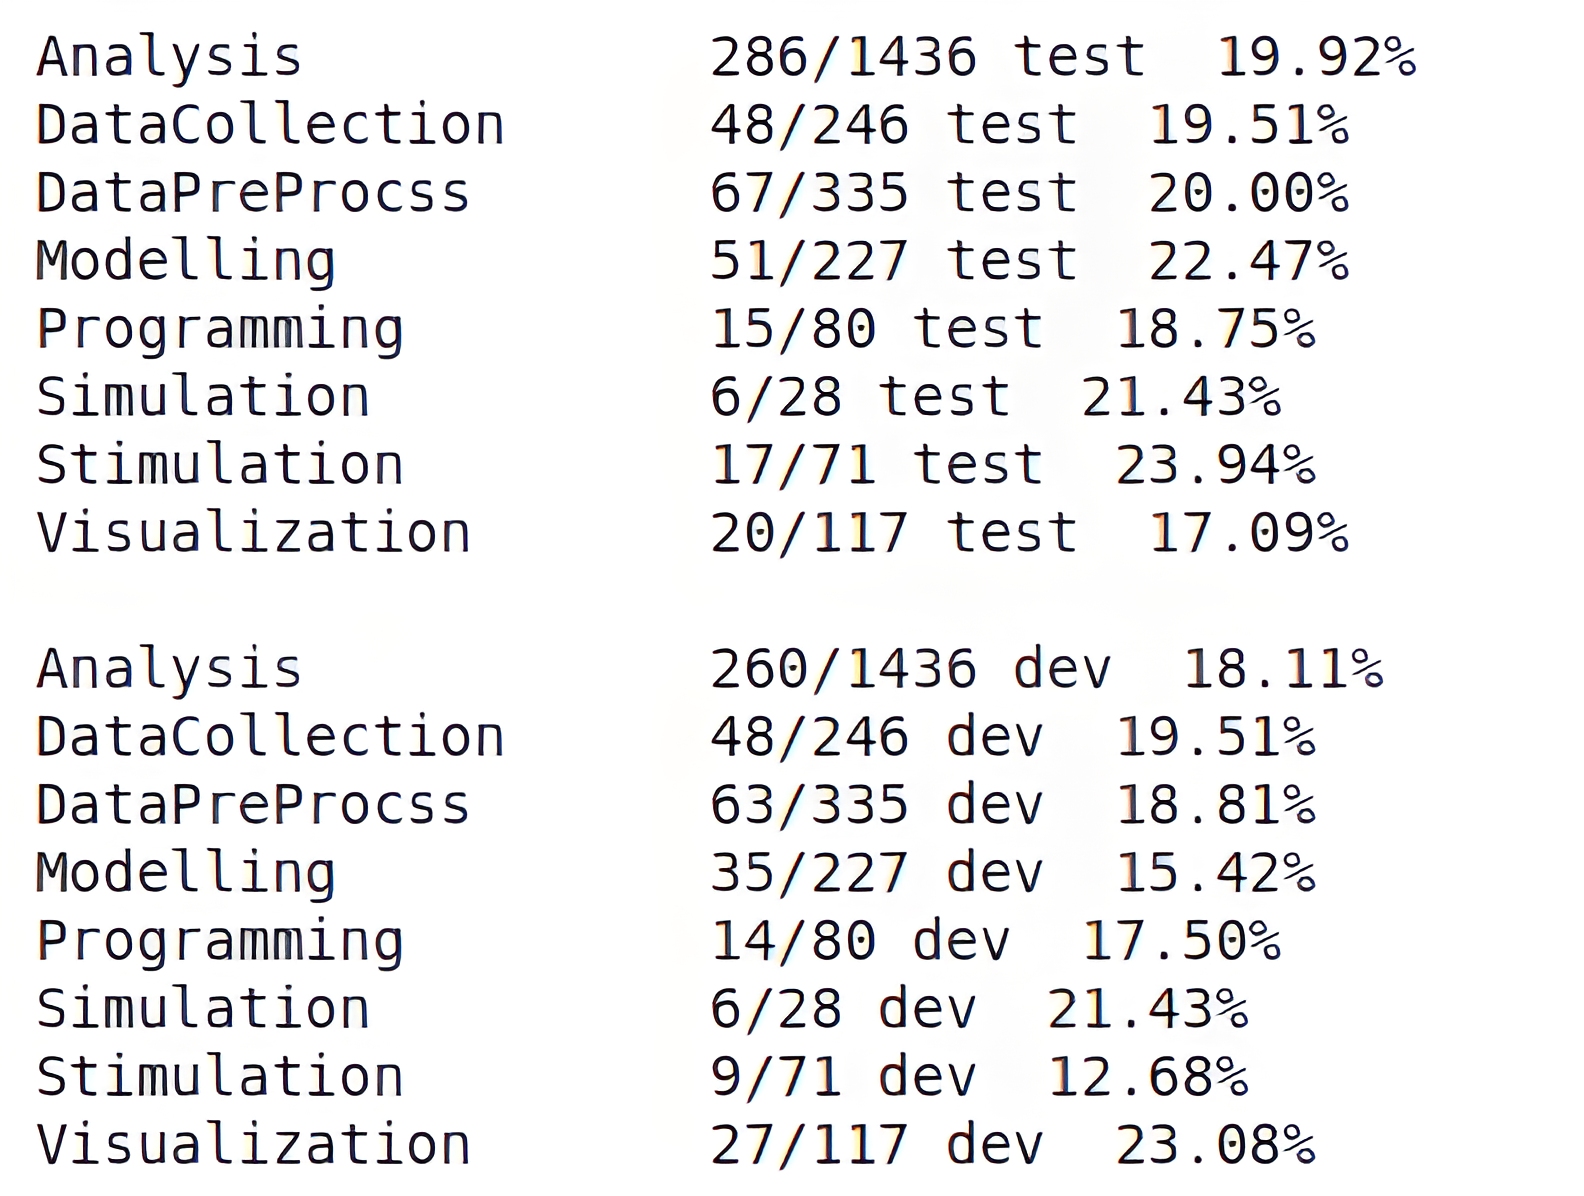
\includegraphics[width=.55\textwidth]{4.graphics/figures/ch_6/optimal_split_sofar}
	\caption{The best data split result before further manual balancing.}
	\label{fig:chapter04:setup}
\end{figure}

Part of a python code for optimizing the data split has been listed on \emph{appendix D}. The notebook for data set splitting and optimization can be found on a git-hub repository  \footnote{\url{https://github.com/BeTKH/SoMeNLP/tree/2layerClassfier/bin}}. 

\section{Model training with inclusion/exclusion part of data}
\label{sec:chapter06:exclusion}

As described in section 4.2.1 before, the SoMeSci dataset is composed of 4 different sets of articles: as \emph{PLoS-methods}, \emph{PubMed-full text}, \emph{ PLoS-sentences} and \emph{creation-sentences}. Since only articles in the  \emph{PLoS-methods} and \emph{PubMed-full text} are annotated with software usage purpose labels, it was desired to evaluate weather including \emph{PLoS} and \emph{Creation} sentences would result in improved performance of the software usage purpose classifier.   \\

The results of evaluation indicates that including \emph{PLoS-sentences} and \emph{Creation-sentences} in the training dataset, definitely improved model performance for classification of software. However, the software purpose classifier’s performance is not improved, rather deteriorated. This makes sense given articles in those sentences do not have software purpose labels. \\

\begin{figure}[htbp]
	\centering
	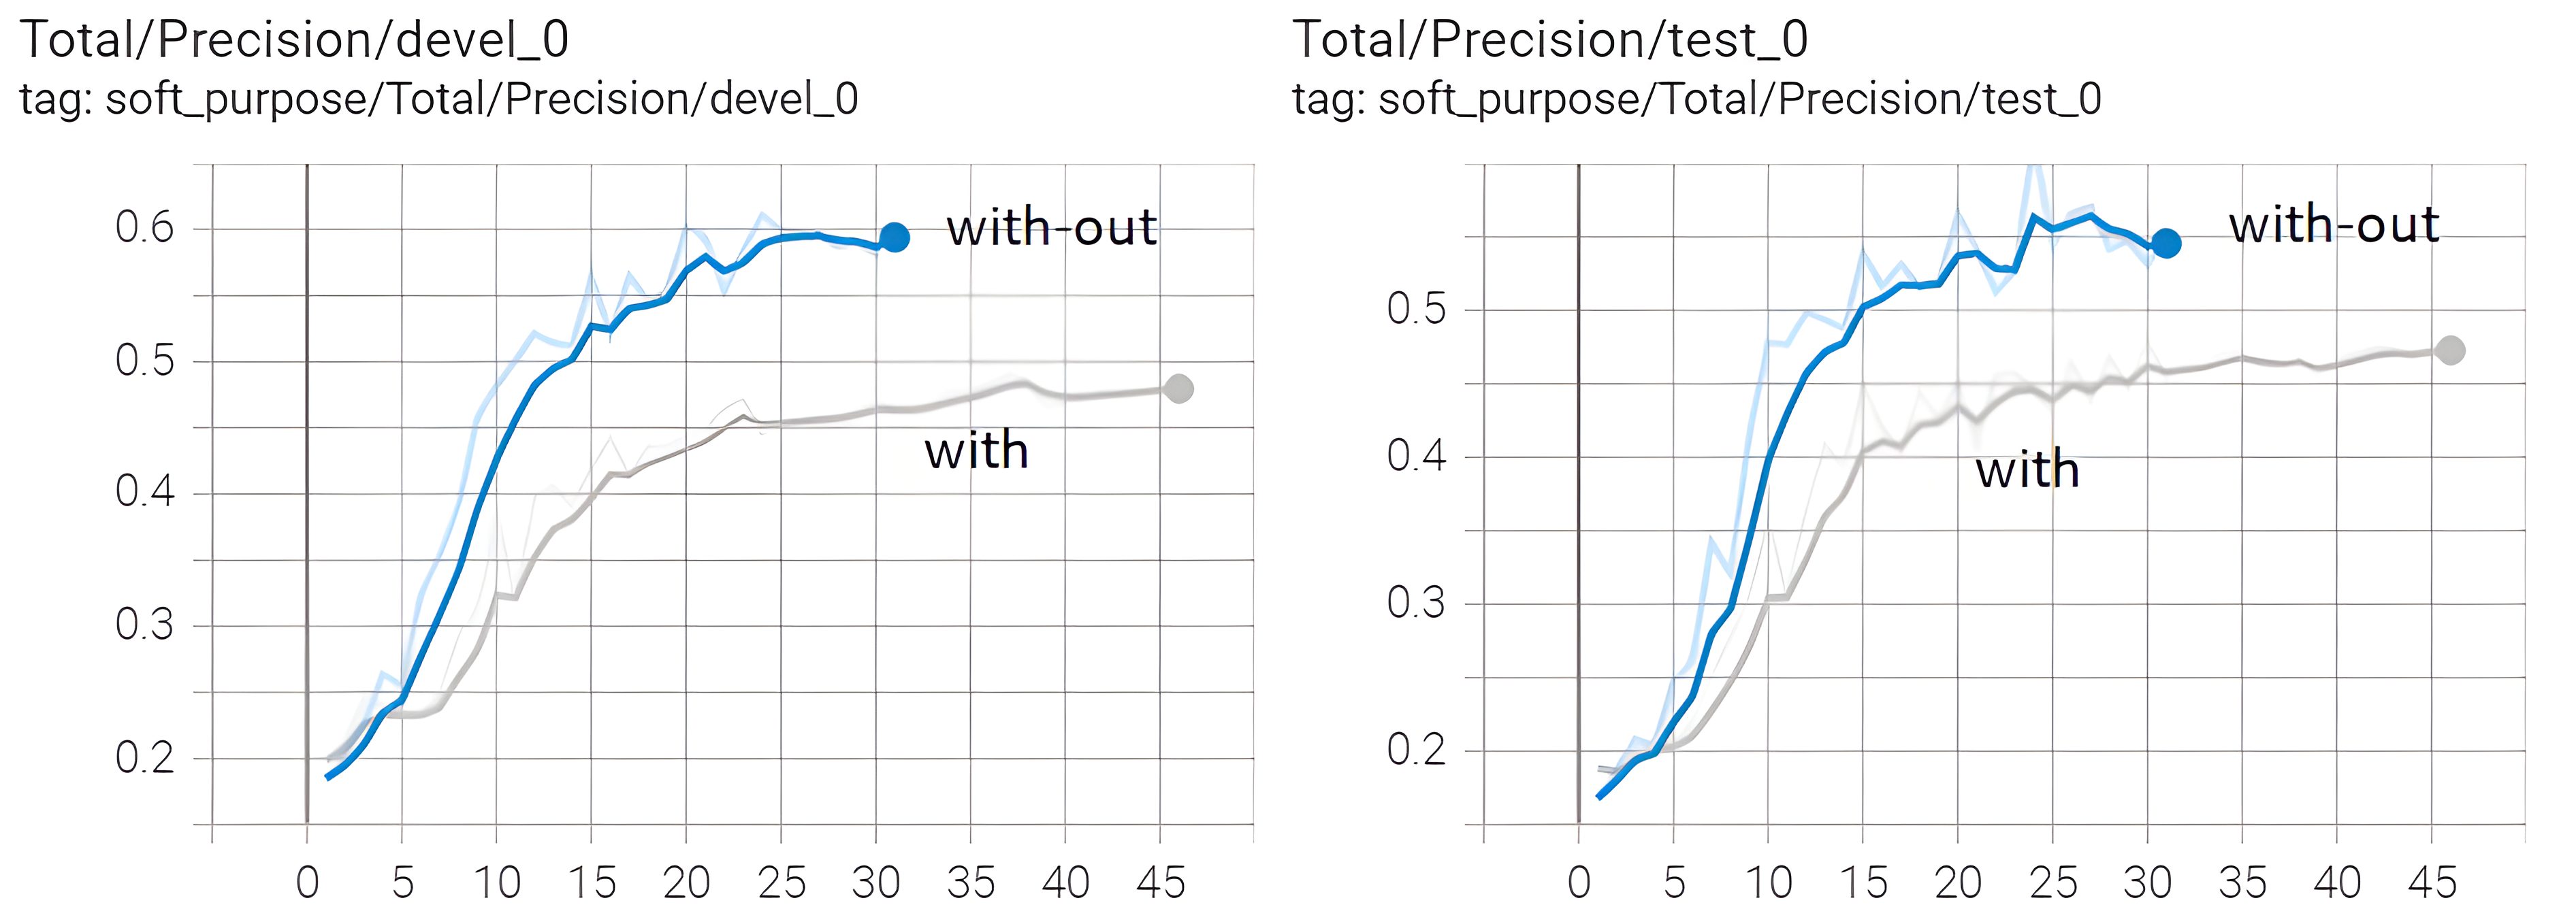
\includegraphics[width=.90\textwidth]{4.graphics/figures/ch_6/1.with_sent_vs_without/HD/1}
	\caption{Software purpose classifier's performance shows improved performance without Creation/PLoS data set.}
	\label{fig:chapter06:without}
\end{figure}


\begin{figure}[htbp]
	\centering
	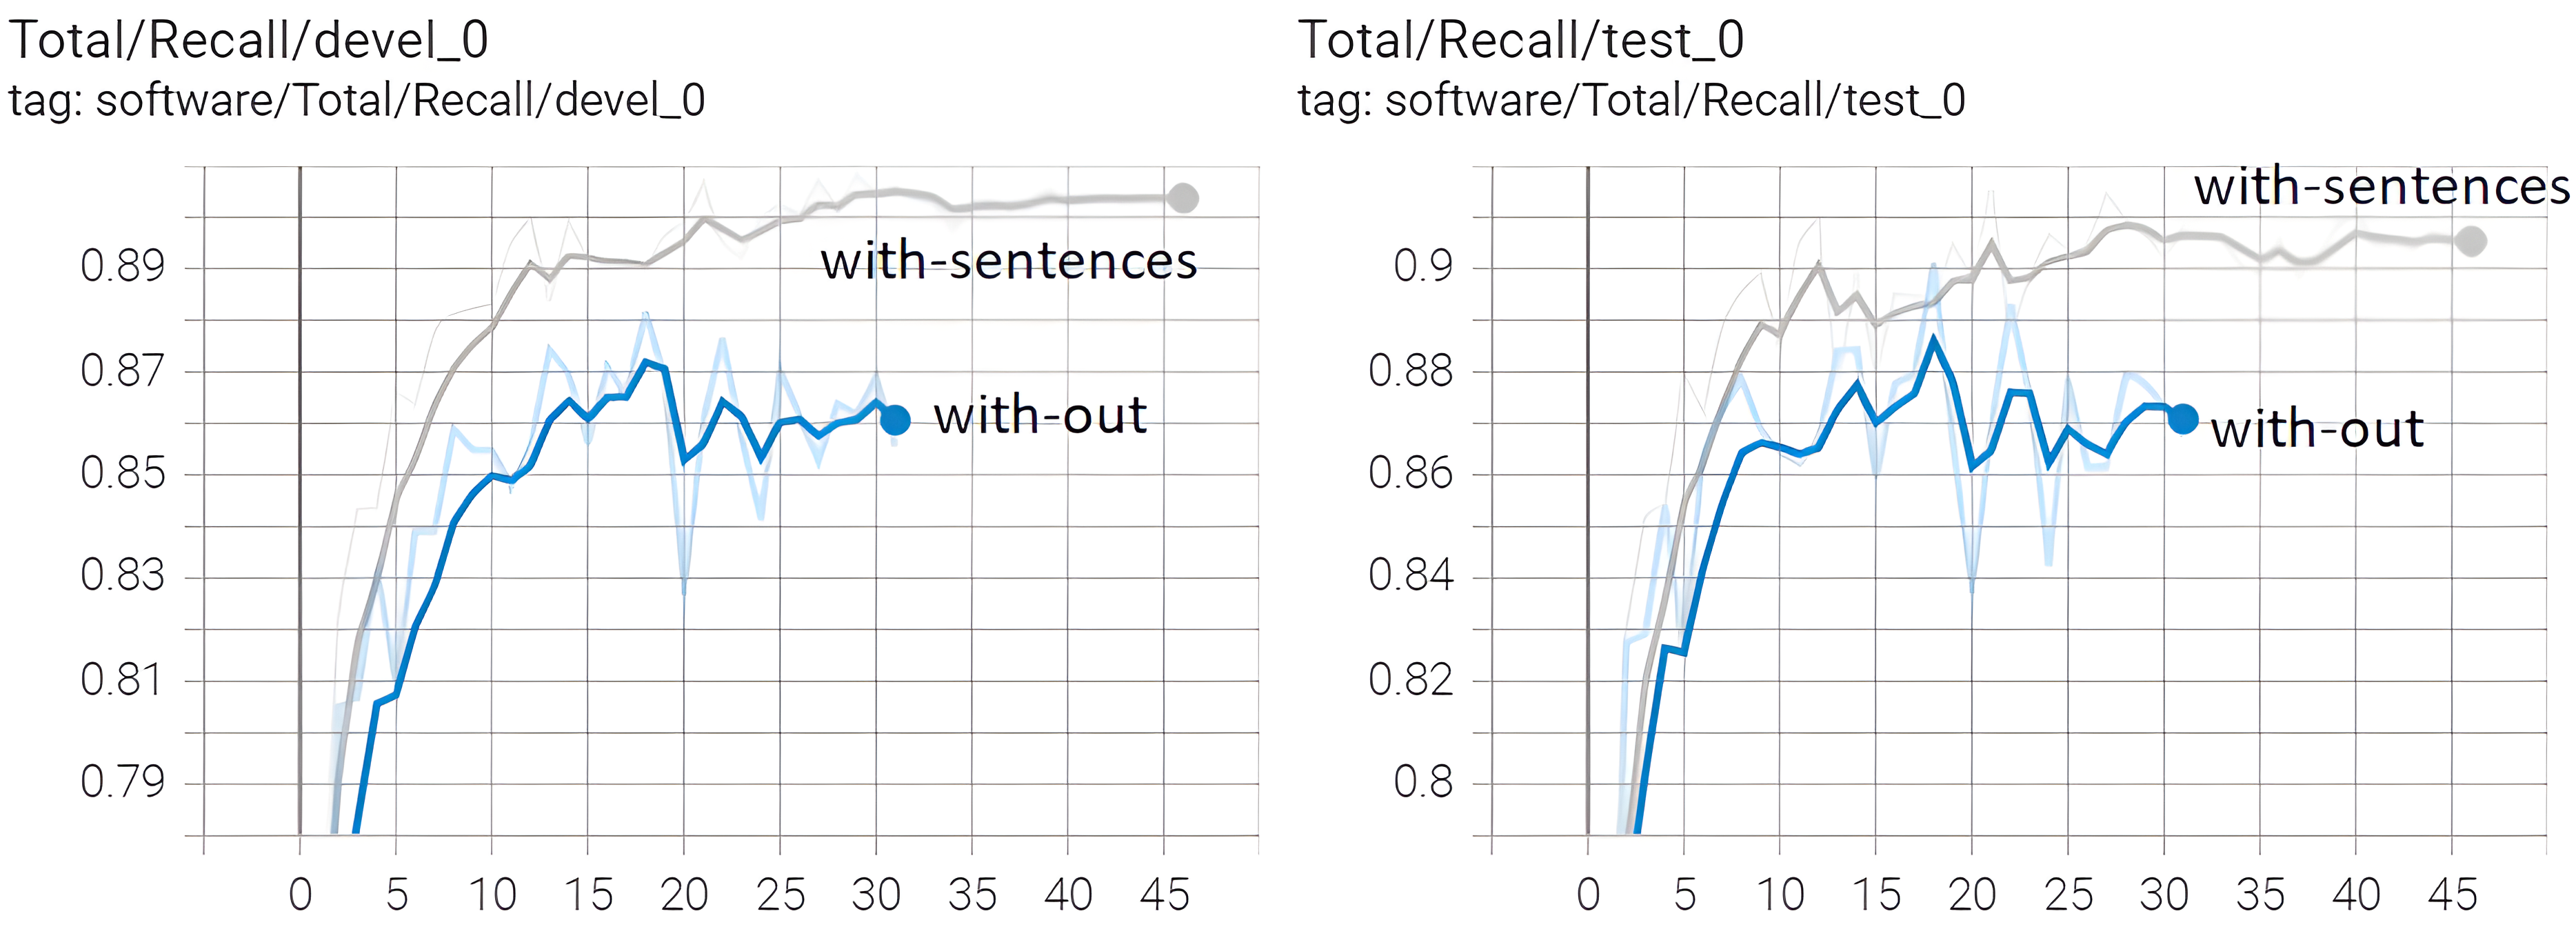
\includegraphics[width=.90\textwidth]{4.graphics/figures/ch_6/1.with_sent_vs_without/HD/2}
	\caption{Software classifier performs better when trained including Creation/PLoS data set.}
	\label{fig:chapter06:with}
\end{figure}

Since the main goal of this project is to maximize software usage purpose classifer’s performance, for subsequent steps of analysis, the software usage purpose classifier has been trained only with datasets of PLoS-methods and PubMed-full text by excluding creation /PLoS sentences. 

\section{The impact of context on classifier’s performance }
\label{sec:chapter06:context}

Scientific papers like any other well written documents, have a sequential structure that form abstraction at various levels such as sentence, paragraphs, sections, chapters, etc. These levels of abstractions often determine the meaning of words because each level of abstraction or context conveys a valuable information \citep{ghosh2016contextual}. \\

Likewise, contextual information helps to determine the correct purpose of use of a software. Therefore for each sentence in a text of scientific articles of training data set, various range of neighboring sentences have been incorporated to provide a contextual information. Typically 2 adjacent sentences before a sentence, after a sentence, and before \& after a sentence have been considered. Further more, a context as broad as the whole paragraph has also been considered. \\

Excerpt of the python code for reading neighboring sentences for context has been listed on the \emph{appendix E}.The complete code has been listed on git-hub inside a methods that reads a file  \footnote{\url{https://github.com/BeTKH/SoMeNLP/blob/contxt2Sentcs_wo/somenlp/NER/data_handler.py}}. 

\subsection{Left Context vs Right Context of Sentence}
\label{sec:chapter06:leftvsright}

Left context refers to sentences prior to a given sentence with in  a paragraph and right context refers to sentences that lie right after a given sentence. \\

Classifier’s performance evaluation indicate that there is a slight improvement in model’s performance for right context as compared to the left context. However, when 2 sentences to left as well as right are taken into account for context, there is no significant gain on the model’s performance for both software and purpose of usage. \\

\begin{figure}[h]
	
	\myfloatalign
	
	\subfloat{
		\label{fig:chapter03:subfloat:grafik1}
		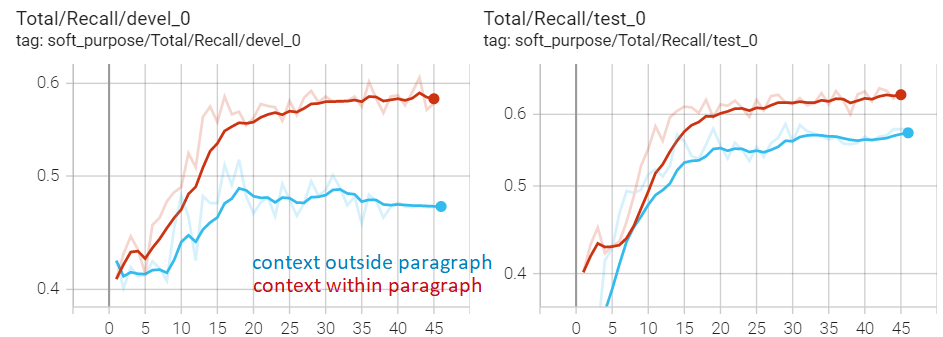
\includegraphics[width=.90\linewidth]{4.graphics/figures/ch_6/2.left_context_vs_right/HD/1}
	} \\
	\subfloat{
		\label{fig:chapter03:subfloat:grafik4}
		\includegraphics[width=.90\linewidth]{4.graphics/figures/ch_6/2.left_context_vs_right/HD/2}
	}\\
	\caption{The effect of context information on software purpose classifier's performance: right context gives improved performance over left context as well as left and right context.}
\end{figure}

Theoretically consideration of broader context, is supposed to improve the classifier’s performance. However, the result of the analysis indicates that a context as big as the whole paragraph did not contribute to the model’s classification performance. Rather, a smaller window of context such as 2 sentences left and right has a better performance. 

\begin{figure}[htbp]
	\centering
	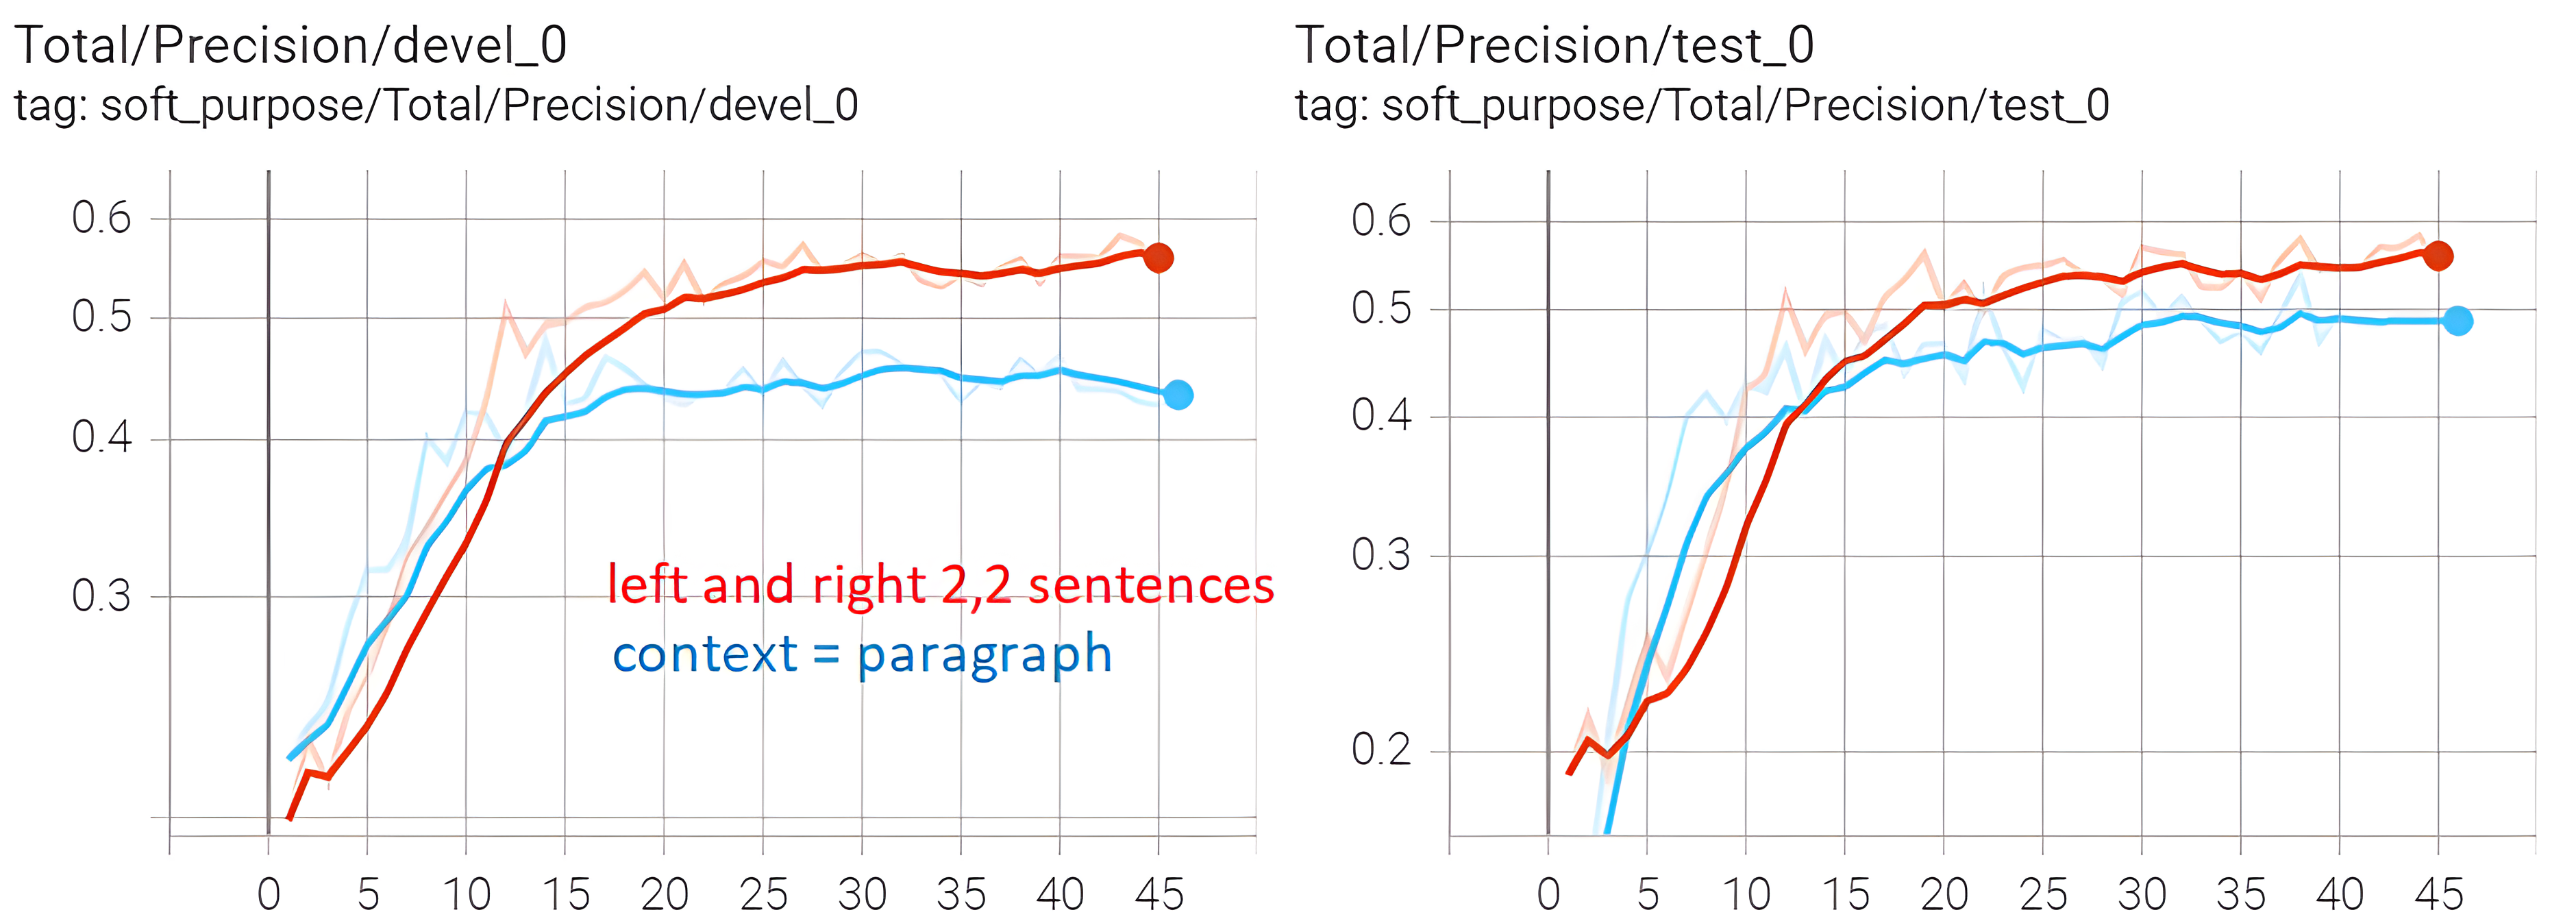
\includegraphics[width=.90\textwidth]{4.graphics/figures/ch_6/3.paragraph_context_vs_22/HD/1}
	\caption{Consideration of broader context leads to loss of classifer's performance.}
	\label{fig:chapter06:with}
\end{figure}


\subsection{Context Outside a Paragraph}
\label{sec:chapter06:contxtOutside}


The other scenario considered was evaluation of model’s performance when context is not limited to a paragraph. The results indicate that, classifier’s performance degraded when a context is not limited within a paragraph. This agrees with the fact that each paragraph of a scientific publication conveys a specific information and a contextual information outside a paragraph might not be useful for the classifier. 

\begin{figure}[htbp]
	\centering
	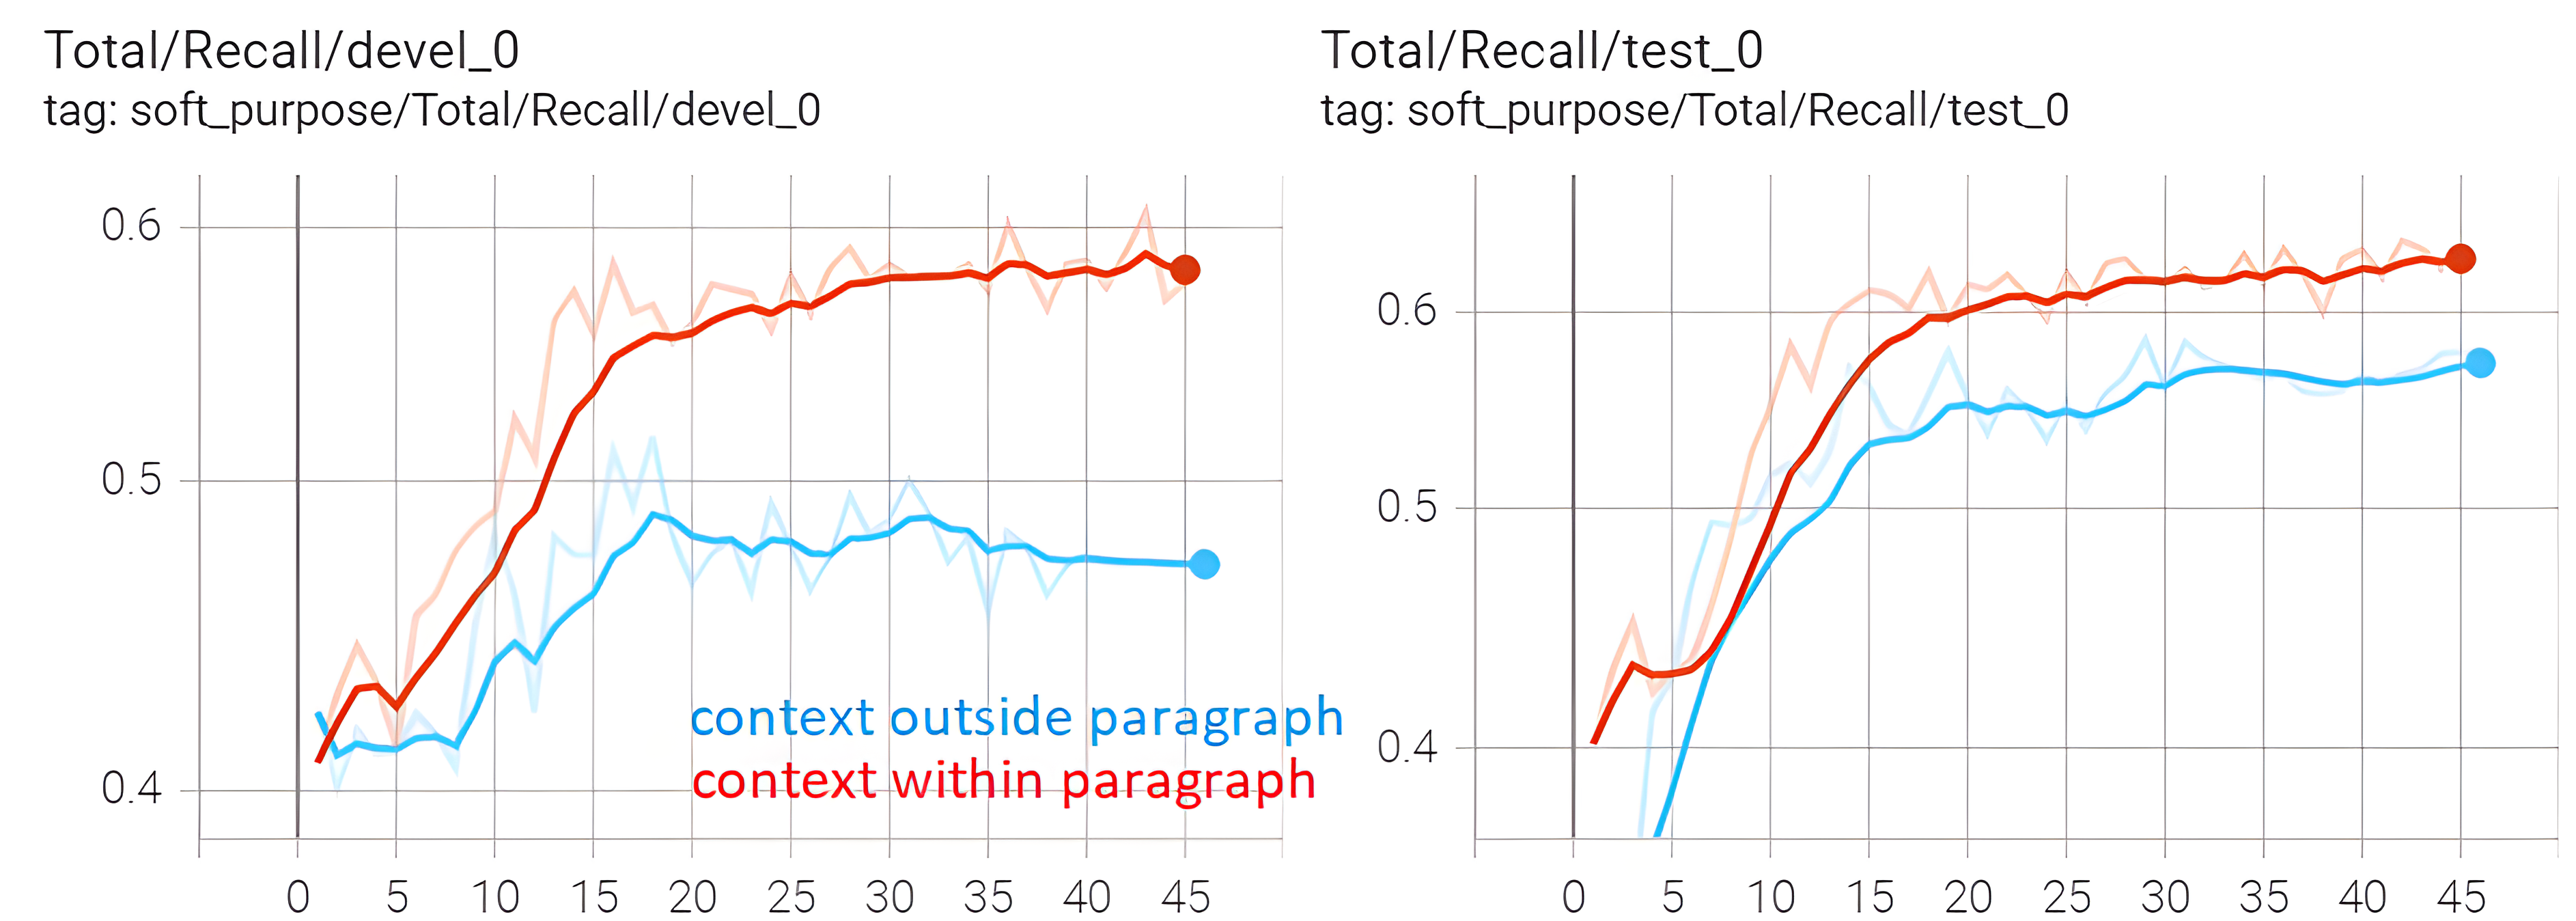
\includegraphics[width=.90\textwidth]{4.graphics/figures/ch_6/4.context_outside_paragraph_vs_inside/HD/1}
	\caption{The impact of context outside a paragraph vs inside.}
	\label{fig:chapter06:with}
\end{figure}

\subsection{Classification with 2-layers}
\label{sec:chapter06:2lc}

Overall the 4-layred \ac{Bi-LSTM-CRF} multi-class classifier’s performance has been poor regardless of consideration of various factors discussed above. Because of this, the model has been simplified into a two layered Bi-LSTM-CRF model by removing software-type and mention-type classifiers. \\

Truncating the model into two layers helped to evaluate the software purpose classifiers performance exclusively by removing the effects of intermediate layers of mention-type and software-tape classifiers. \\

\begin{figure}[htbp]
	\centering
	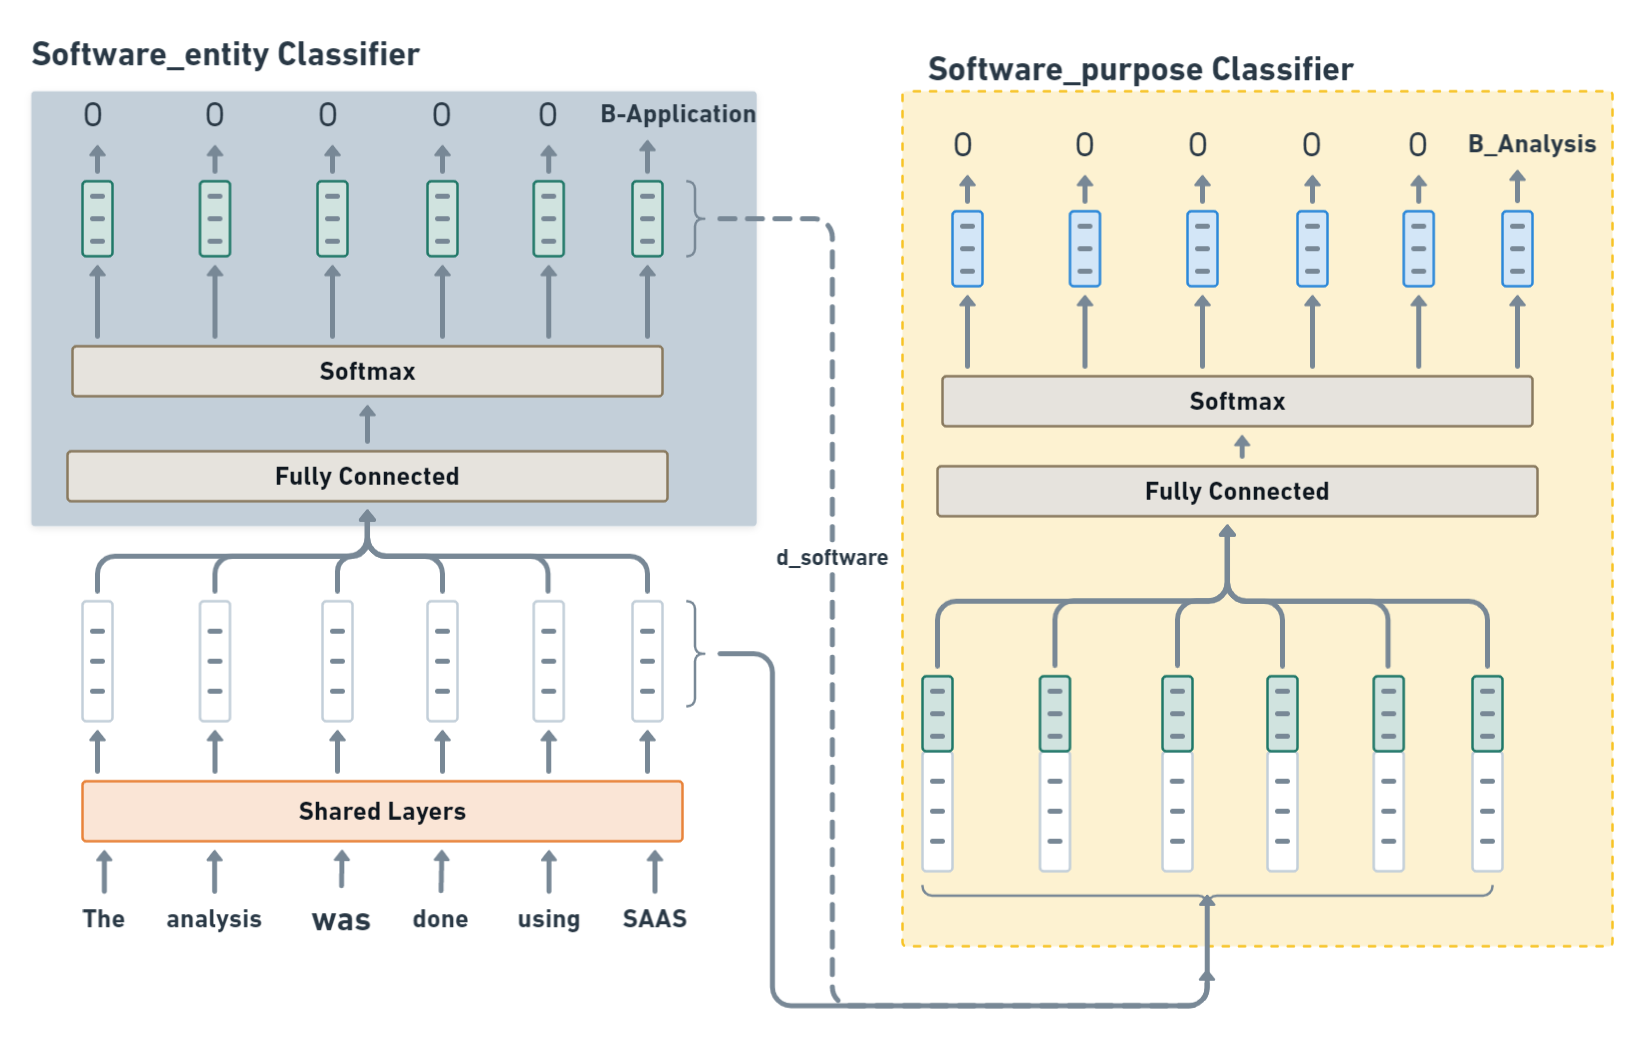
\includegraphics[width=.90\textwidth]{4.graphics/figures/ch_5/2LC}
	\caption{Two layered classifier fully connected model.}
	\label{fig:chapter06:with}
\end{figure}

Evaluation of the 2-layered classifier model reveals that overall software purpose classification performance has shown small improvement compared to the original 4-layered \ac{Bi-LSTM-CRF} model, where as the software classifier’s performance does not indicate any performance improvement.  

\begin{figure}[h]
	
	\myfloatalign
	
	\subfloat{
		\label{fig:chapter03:subfloat:grafik1}
		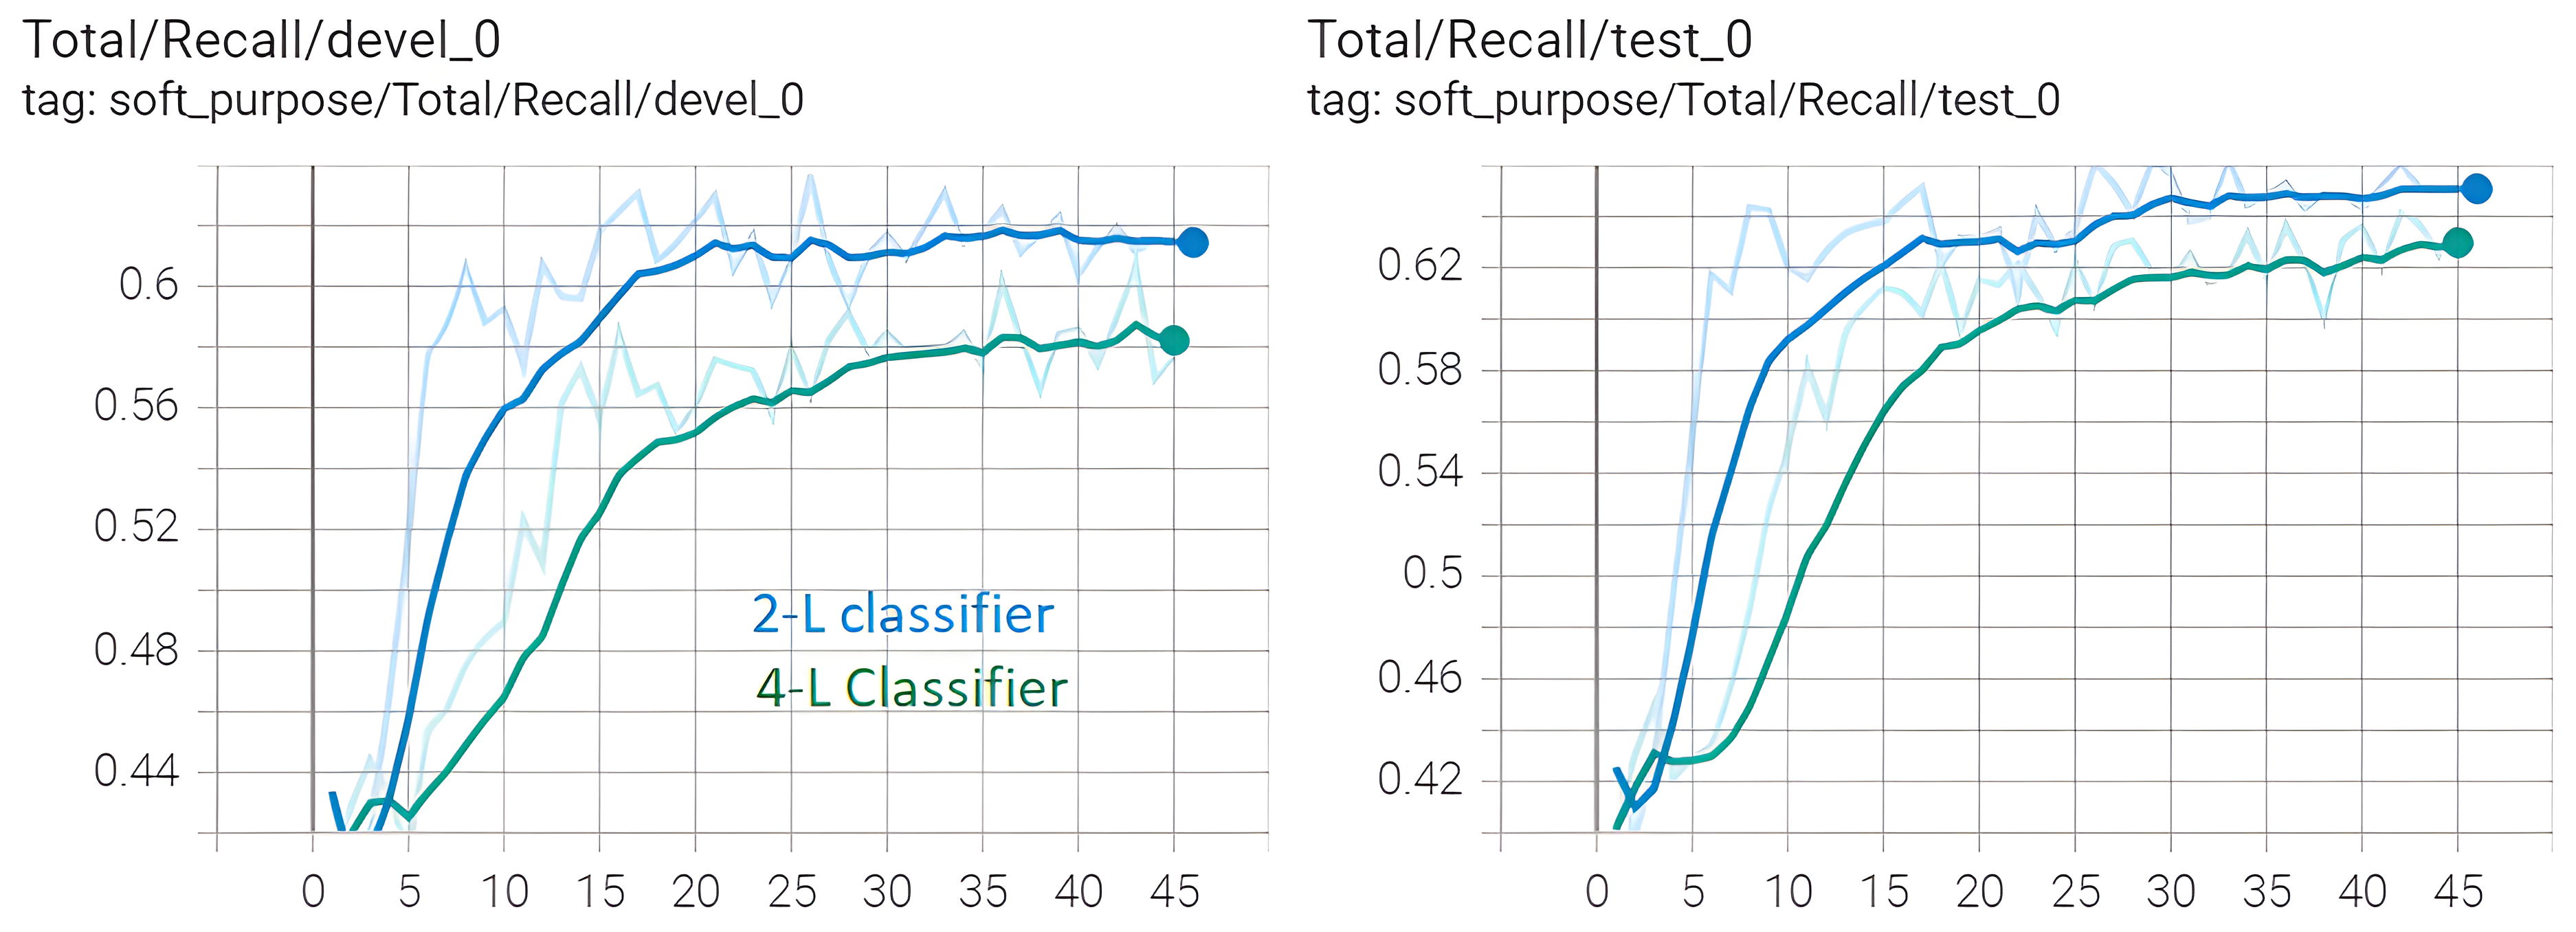
\includegraphics[width=.90\linewidth]{4.graphics/figures/ch_6/5.2layerClassifier/HD/1}
	} \\
	\subfloat{
		\label{fig:chapter03:subfloat:grafik4}
		\includegraphics[width=.90\linewidth]{4.graphics/figures/ch_6/5.2layerClassifier/HD/2}
	}\\
	\caption{The Truncated 2-layer \ac{Bi-LSTM-CRF} classifier performed slightly better compared to the 4 layered model.}
\end{figure}


\section{Model Training Bio-BERT vs Sci-BERT}
\label{sec:chapter06:biosci}

Even though both \ac{Bio-BERT} and \ac{Sci-BERT} give a contextualized representation of a word in a sentence, representations of a word would differ due to the inherent difference of corpora used for pre-trained models of Bio-BERT and Sci-BERT \citep{beltagy2019scibert,li2019fine}. For this reason, classifier’s performance has been evaluated for both Sci-BERT and Bio-BERT models. \\

The results of evaluation indicate that the classifier models performed slightly better when using Bio-BERT large embedding compared to Sci-BERT. However, the model performed better with Sci-BERT compared to the Bio-BERT small embedding. 

\begin{figure}[htbp]
	\centering
	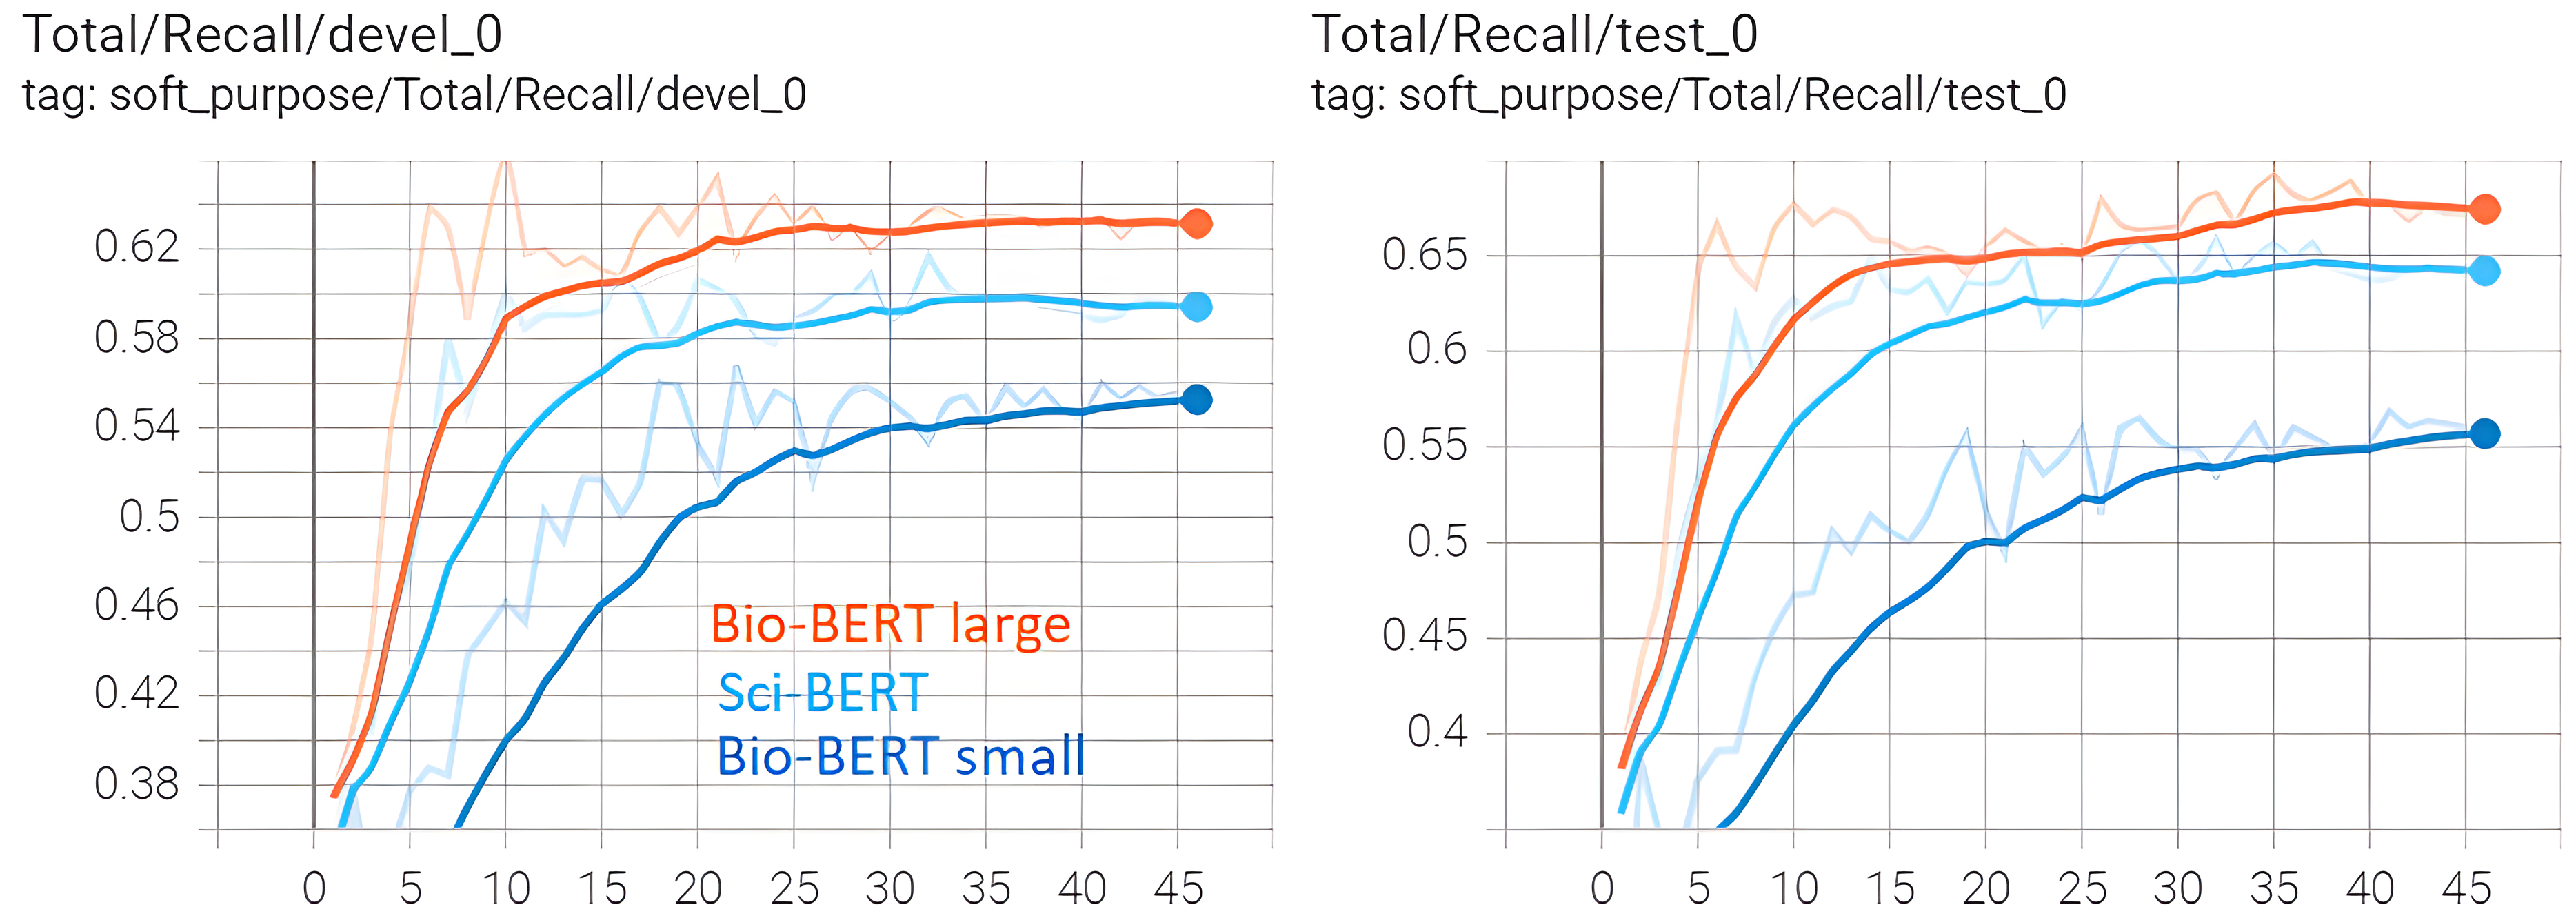
\includegraphics[width=.90\textwidth]{4.graphics/figures/ch_6/6.BIoBERT_vs_SCIBERT_2LAYER_Classifier/HD/1}
	\caption{Two layered classifier fully connected model.}
	\label{fig:chapter06:with}
\end{figure}

\section{Summary of Training Results }
\label{sec:chapter06:summary}

Performance evaluation of the Bi-LSTM-CRF multi-class classifier model, in various training scenarios, reveals some interesting insights. \\

Firstly, the analysis of the model performance results indicate that, the composition of the data set has significant impact on the models performance. As stated before, when the classifier model is fed with data set that lacks software purpose annotations in creation and plos sentences, the models performance decreased. \\

Secondly, it has been observed that various levels of context can affect models performance. As presented earlier, when neighboring sentences in a scientific articles of SoMeSci data set is considered it has been clearly observed that models performance has shown improvement. However, the analysis also reveals that unbounded context information such as a context outside a given paragraph is not useful to the model’s performance, rather it will degrade the models performance. Further more, it has been observed that a context of sentences on the left and right might not be equally important. The analysis results indicated that a context of sentences from the right were observed to be more useful to the models performance that the left. \\

Thirdly, evaluation of the classifier’s performance by truncating the intermediate layers of classifiers indicated a marginal improvement of software purpose classifier which lies at the end of the 4-layered chain of classifiers but there was no tangible performance gain was observed for the software classifier. This might indicate that, probably there flawed classifications of intermediate layers might have an impact on the software purpose classifier. \\

Further, it was also observed that the use of various types of embeddings like Bio-BERT and Sci-BERT impacted the classifier’s performance. The use of larger variants of embedding models was observed to improve classifiers performance. \\

Ultimately, it is reasonable to conclude that the study of all training scenarios and consideration of factors does not show a very large scale performance gain or loss. This might be because a constraint on the amount of labeled data set and unavailability of larger size of training data set. 



\subsection{Summary of Software Purpose Classifier performance}
\label{sec:chapter06:summary_softPurpose}

\subsection{Summary of Software Classifier performance}
\label{sec:chapter06:summary_soft}



















